\section{Подбор оптимального размера конечного элемента}

Было построено 7 моделей с различным размером конечного элемента. Путем расчета моделей с заданными нагрузками были определены средние величины напряжений для стенок в наиболее напряженных отсеках (обозначены белым на  Рис.\ref{fig:WingRootPlain})

\begin{figure}[ht]
\centering
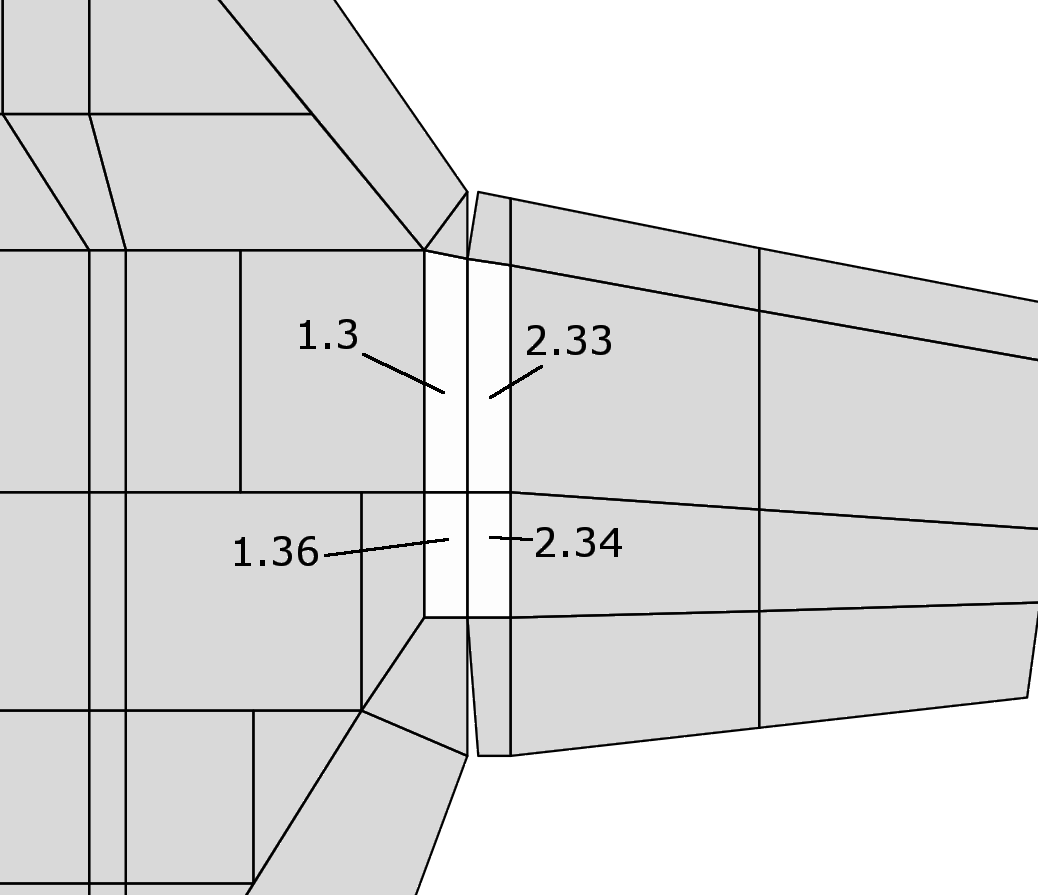
\includegraphics[width=0.6\textwidth]{RootOfWingWithSelectedPartsBW}
\caption{Стык правого крыла и фюзеляжа. Схематичное изображение вида сверху}
\label{fig:WingRootPlain}
\end{figure}


\begin{figure}[H]
\centering
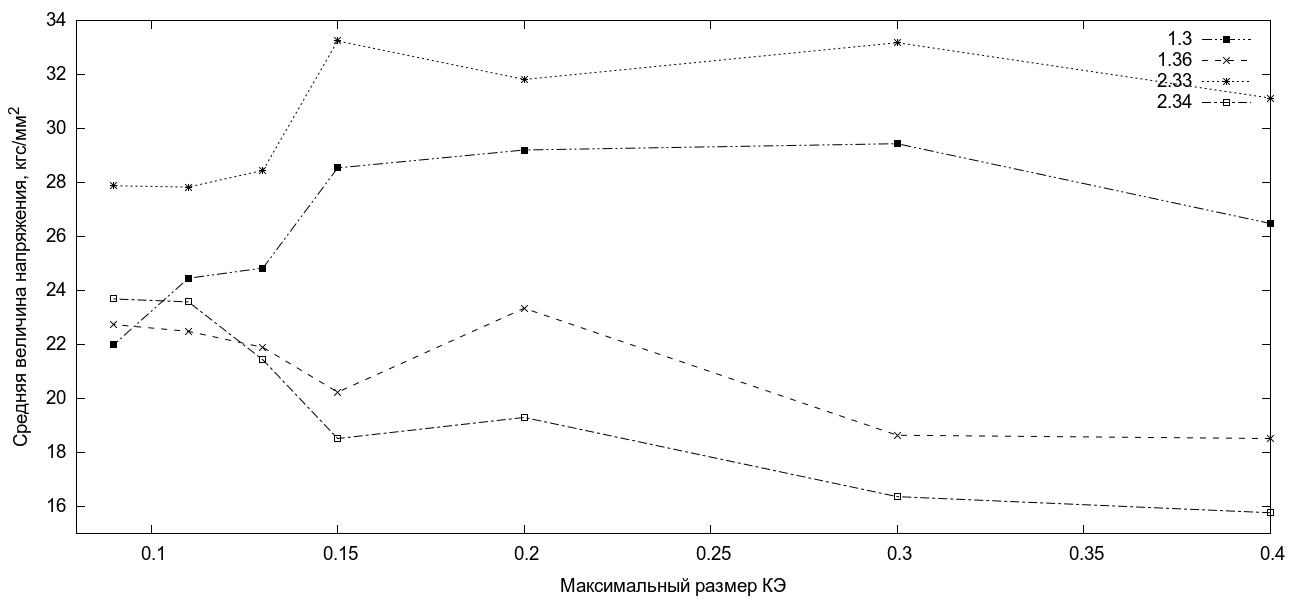
\includegraphics[width=0.8\textwidth]{StressToDiscretenessPlot}
\caption{Зависимость средних напряжений в отсеках от величины КЭ}
\label{fig:stressToDiscreteness}
\end{figure}

Была получена зависимость средних напряжений в этих отсеках от размера конечного элемента (Рис.\ref{fig:stressToDiscreteness})

На основании полученных данных была определена оптимальная величина конечного элемента для дальнейшей работы над моделью, равная $0,11\text{м}$. 
%Ниже приведены картины НДС в месте стыка крыла с фюзеляжем при различных размерах конечного элемента. 